\newcommand{\myabstract}{
\noindent Do people reward (RTM) or shoot the messenger (STM)? In two preregistered
experiments (N=5,200), a participant---the respondent---performed a task for
real money. Another person---the messenger---told the respondent whether
they succeeded or failed. Next, participants were matched with a partner---either the messenger or another participant. Using economic games, we measured
how prosocial respondents were toward their partner. Using rating scales, we
measured how much they liked their partner. In Experiment 1, we find both an STM
and an RTM\@. Moreover, good or bad news did not affect how respondents treated
non-messengers. In Experiment 2, we informed respondents that messengers had no
stakes in the news or earned money when participants succeeded or failed. When
messengers had no stakes in the outcome, respondents rewarded messengers when
they succeeded. When messengers had a stake in respondents' success (failure),
the STM disappeared (was exacerbated) whereas the RTM persisted.}
\clearpage

\begin{abstract}
    \myabstract
    
    \vspace{0.2in}
    \noindent \textbf{Key Words}: voter turnout; emotions; anger; field experiments\\
    \noindent \textbf{Word Count}: 11,691
    \end{abstract}
    \clearpage

\begin{epigraph}
  {How beautiful on the mountains are the feet of those who bring good news.}{Isaiah 52:7}
\end{epigraph}
  
\begin{epigraph}
  {Nobody likes the man who brings bad news.}
  {Sophocles, Antigone, Scene I, 233}
\end{epigraph}

\vspace{.5cm}

Do people treat messengers differently depending on whether they deliver
good or bad news? History offer many examples of
messengers being rewarded after bringing good news or falling in
disgrace after bearing bad news. One famous example includes
Pheidippides, who was hailed as a hero after announcing Athens' victory
in the battle of Marathon and exhaling his last breath after running 42
kilometers to deliver the news \citep{christensen2009herodotosa}.

\emph{Messenger bias}, i.e., people's tendency to reward messengers for
bringing good news and punish them for breaking bad news, is present
also in modern life and has implications for better understanding
interpersonal relationships, workplace interactions, and
politics.\footnote{Although ``messenger bias'' may encompass the
  disparate treatment of messengers on the basis of gender, race, or
  other demographic characteristics, this paper focuses on the messenger
  bias due to the valence of message content.} The inefficiencies and
large societal costs caused by this messenger bias invite studying it
and understanding how to ameliorate it. When messengers expect a bias
depending on the news they bear, whether it is positive for good news or
negative for bad news, they may act in anticipation of those effects.
For instance, employees who fear punishment for breaking bad news to
their managers may prefer to stay quiet (i.e., shooting the messenger),
threatening corporations' long-term survival \citep{charan2002companies}.
Similarly, in the wake of a disaster, politicians may downplay
responsibilities \citep{liu2020framing}, hindering efforts to prevent the
next catastrophe. At the same time, the opposite side of the messenger
bias may be just as detrimental. Rewarding the messenger who brings good
news may lead employees and politicians to focus on finding ways to be
the ones who \emph{communicate} good news rather than those who
\emph{work} toward achieving good outcomes \citep[see, e.g.,][]{grimmer2014impression}.
Throughout this paper, we label the ``shoot the
messenger'' effect as the ``STM'' effect and the ``reward the
messenger'' effect as the ``RTM'' effect.

We provide the first experimental demonstration of messenger bias using
behavioral outcomes and also confirm and extend prior results found with
attitudinal measures. We also show how the messenger bias
can be reduced. In our experiments, we use real human participant to
both receive messages and to deliver messages, a point of contrast from
prior work using confederates or a fictional character in a vignette \citep{kuhlen2013language}. 
In two large pre-registered experiments (Study 1 and Study 2), we compared
people's decisions toward a messenger who delivered good rather than bad
news against decisions toward another partner who was not the messenger.
\footnote{The pre-registration for Study 1 can be found at \url{https://aspredicted.org/PD3_KC2}, 
and the pre-registration for Study 2 can be found at 
\url{https://aspredicted.org/8TG_4KY}.} 
 In
the second study, we also manipulate the messenger's payoffs depending
on the news they delivered and fully informed participants of the
messenger's incentives. The messenger earned (lost) money when the
respondent won (lost) (shared fate), lost (earned) money when the respondent
won (lost) (opposite fate), or earned nothing regardless of the outcome
(unrelated fate). In both experiments, we informed the subject that the
messenger had no control over the outcome news that they transmitted and
they delivered the news simply by clicking a button.

\begin{table}[]
\caption{Summary of our results regarding messenger bias}
\centering
\scalebox{.75}{%
\begin{threeparttable}
\begin{tabular}{@{}lll@{}}
\toprule
 & RTM & STM \\ \midrule
Study 1 (Baseline Study) & \makecell[l]{Present for some behaviors\\and all attitudes} & \makecell[l]{Present for some behaviors\\and all attitudes} \\
Study 2 (Adding Incentive Conditions) & \makecell[l]{Eliminated by unrelated fate condition\\(but only for behaviors)} & \makecell[l]{Eliminated by all fate conditions,\\and shared fate reverses it for behaviors} \\ \bottomrule
\end{tabular}%
\begin{tablenotes}[flushleft]
\scriptsize{\item[\hspace{-5mm}] \textit{Note:} Our experiments measure both behavioral outcomes and attitudinal measures. Behavioral measures include the dictator game, spin the wheel task, and the prisoner’s dilemma. Attitudinal measures include partner ratings of trustworthiness, likeability, niceness, and generosity.}
\end{tablenotes}
\end{threeparttable}
}
\label{tab:summary-results}
\end{table}

We find three new results across Studies 1 and 2, as summarized in 
Table \ref{tab:summary-results}. First, in both of our
studies, we confirm the existence of the shoot the messenger (STM)
effect, while also discovering a reward the messenger (RTM) effect. The
RTM effect is as large, if not larger, than the STM effect across both
Study 1 and Study 2. Second, we examine the implications of the
messenger bias by using behavioral measures, in addition to the
attitudinal measures that previous research has exclusively focused on.
We find that although in this context attitudinal effects appear to
correlate with behavioral outcomes, attitudinal measures overestimate
the messenger bias compared to behavioral measures. Finally, when
varying the incentives of the messenger in Study 2, we discover that
merely specifying the incentives of the messenger eliminates the STM for
both behaviors and attitudes, while the RTM effect remains remarkably
durable across various treatment conditions. Therefore, we contribute a
partial remedy that can help avoid the adverse consequences of messenger
bias in everyday life.


\emph{Messenger bias} measures how a messenger is treated as a
consequence of merely delivering a message. One side of the messenger
bias, the STM effect, has been assumed in prior work, which investigated
how belief in punishment for delivering bad news affected behavior.
Specifically, the antecedent of the messenger bias is the MUM (Mum about
Undesirable Messages) effect, which is the notion that people are
typically more reluctant to convey bad news than good news \citep{rosen1970reluctance,rosen1972fear}. 
Messengers prefer to avoid conveying bad news
because they fear backlash, especially when in public \citep{bond1987reluctance}.
 Later work found that this effect applies to a myriad
of situations in everyday life, such as doctors to patients \citep{clark1982death, sheldon1982truth, taylor1988telling}
 or politicians to voters \citep{dorling2002good,levy2014soothing}.

There is limited work directly demonstrating that messengers receive
biased treatment when they merely deliver good or bad news. The prior
work that is closest to our research is ``Shooting the Messenger''
\citep{john2019shooting}, which focused on people's dislike for messengers
who break bad news to them. Across several experiments, the authors
randomly assigned participants to receive good or bad news from a
research assistant who acted as a messenger. After they learned that
they won (if an odd number was randomly drawn) or lost, participants
rated the messenger's likeability on a 10-point scale. In other
experiments, the authors isolated several features of the STM effect:
the effect was specific to the messenger (compared to non-messengers),
was amplified when bad news was unexpected, and was mediated by
self-reported perceptions that the messenger had malevolent motives.
Finally, when the authors manipulated whether the messenger's motives
were aligned or misaligned with the participant's (but without a neutral
alignment condition), subjects reported that they liked shared alignment
messengers delivering bad news more than misaligned ones. Separately,
the same paper also found initial evidence that people like messengers
who bring good news, although they did not explicitly identify a RTM
effect.

Several explanations have been offered for the messenger bias. As \citet{john2019shooting}
 found, the respondent may shoot the messenger for bringing
bad news by assuming them to have malevolent motives or in a desire to
make sense of the news by blaming the messenger as the most proximate
cause. One relevant set of studies have established that criticisms, or
negative news, from out-group members are treated more harshly compared
to those by in-group members (the intergroup sensitivity effect)
\citep{hornsey2002it,esposo2013shooting}. Therefore, messengers who
bring bad news may be penalized if they are assumed to be acting counter
to the interests of the group. At the same time, this implies that
clarifying the relationship between the messenger and the recipient of
the message may be a fruitful strategy to ameliorate the messenger bias.
Specifically, the messenger showing themselves to be unaligned with any
potential out-groups may reduce the negative effect of criticisms
\citep{hornsey2007groupdirected}.

\begin{table}[]
\caption{Comparison of our work and \citet{john2019shooting}}
\label{tab:previous-work}
\resizebox{\textwidth}{!}{%
\begin{threeparttable}
\begin{tabular}{@{}lll@{}}
\toprule
 & Behavioral Measures & Attitudinal Measures \\ \midrule
Shoot the Messenger Effect & Present Research & Exp. 1, 2A, 2B, 3A, 3B, 4, 5A, 5B, 5C, 6A, 6B \citep{john2019shooting} \\
Reward the Messenger Effect & Present Research & Exp. 2A (N = 150) and 5A (N = 304) \citep{john2019shooting} \\ \bottomrule
\end{tabular}%
\begin{tablenotes}[flushleft]
\scriptsize{\item[\hspace{-5mm}] \textit{Note:} Although one experiment (2A, N=150) in John et al. (2019) did include a 2 x 2 design varying a messenger vs. a non-messenger and good vs. bad news like our experimental conditions, they do not calculate the RTM effect nor is the study well-powered to detect differences between the STM and RTM effects. The other experiment (5A, N = 304), does include a neutral message condition to assess valence effects, but no non-messenger conditions necessary to measure the STM and RTM effects.}
\end{tablenotes}
\end{threeparttable}
}
\end{table}


Taken together, the research on the STM effect and the MUM effect
suggests that messenger bias can impose tangible costs on modern society
because messengers who tell bad news are disliked and thus prefer to
stay quiet. Table \ref{tab:previous-work} summarizes the prior work and shows how our work
contributes the current literature in two ways.


Several important questions remain unaddressed in prior work. First, it
remains unknown whether attitudes toward the messenger are accompanied
by behavioral consequences. Prior work measured
\emph{attitudes} toward the messenger (especially
likeability and competence). Ultimately, uncovering whether messengers'
news may affect altruism, cooperation, and trust toward them carries
fundamental implications for understanding the information environment.
It remains unknown whether messengers' reluctance to speak out is
justified by actual repercussions against them that go beyond mere
dislike. Previous literature indicates that behavior does not
necessarily track attitudes when it interferes with self-interest and
financial incentives \citep{crano2006attitudes,lehman2002pervasive}.
(And, in equilibrium, the tendency to obscure bad news means that it is
less frequently observed, making it difficult to generate unbiased
inferences about the effect of sending bad news for non-experimental
observations.) In this paper, we address this question and build upon
\citet{john2019shooting} by studying how people treat messengers after
receiving good news or bad news from them using incentivized
experiments. Since we have both behavior and attitudinal measures in the
same studies, we can directly compare the performance of these measures.

Second, our experimental design addresses some issues in prior work.
Such work does not fully identify the composition of the messenger bias
because of their experimental designs, which only compare reactions to
messengers bringing bad news to messengers bringing good news. Our paper
adds a ``messenger vs. non-messenger'' condition to all our
experiments in addition to the ``good news vs. bad news'' conditions.
This allows for two benefits. First, we more accurately identify the
\emph{shoot the messenger} effect (i.e., the negative reaction to a
messenger delivering bad news compared to a non-messenger) as something
distinct from the \emph{valence} effect (i.e., the negative reaction to
receiving bad news generally compared to receiving good news). Because
previous studies do not distinguish between these two effects, it
remains unclear whether there is something distinct about the
\emph{delivery} of bad news which is specific to the messenger from just
bad news generally. The second benefit is the ability to estimate the
opposite side of the messenger bias: rewarding the messenger for
delivering good news. Although previous work has not pointed out the
existence of a RTM effect, perhaps because they assume it to simply be
symmetric to the STM effect, we compare the magnitude and persistence of
these two effects. The Methods section details how we define and analyze
these quantities of interest differently from past work.

\section{Results}

\begin{figure}  
\centering{
\resizebox{1\textwidth}{!}{
\begin{tikzpicture}
\node (r1) [draw=black, dashed, fill=lightgray!30, minimum width=8.15cm,minimum height=7.5cm] at (9,0){};
\node (r3) [draw=black, dashed, fill=lightgray!30, minimum width=4.25cm,minimum height=7.5cm] at (16.5,0){};
\node (r1Label)[above=.67cm of r1] {\textbf{Part 2: Behavioral Games}};
\node (r2) [draw=black, dashed, fill=lightgray!30, minimum width=1.75cm,minimum height=7.5cm] at (3,0){};
\node (r2Label)[above=0cm of r2] {\textbf{  \begin{tabular}{c}
     Part 1: Perform Task\\
     and Receive Message\\
  \end{tabular} }};
\node (r3Label)[above=.58cm of r3] {\textbf{After Part 2 Complete}};
\node[shape=rectangle, draw] at (0,0) {SUBJECT};
\node[shape=rectangle, draw,  align=left] at (3,2) (win) {Win\\Message};
\node[shape=rectangle, draw,  align=left] at (3,-2) (loss) {Loss\\Message};
\node[shape=rectangle, draw, align=left] at (6,3) (messenger_win) {Play with:\\Messenger};
\node[shape=rectangle, draw, align=left] at (6,1) (stranger_win) {Play with:\\Stranger};
\node[shape=rectangle, draw,  align=left] at (6,-1) (messenger_loss) {Play with:\\Messenger};
\node[shape=rectangle, draw, align=left] at (6,-3) (stranger_loss) {Play with:\\Stranger};
\node[shape=rectangle, draw] at (10,3) (bg) {\textbf{Behavioral Measures}};
\node[shape=rectangle, draw] at (10,2) (dg) {Dictator Game};
\node[shape=rectangle, draw] at (10,0) (stw) {Spin the Wheel};
\node[shape=rectangle, draw] at (10,-2) (pd) {Prisoner's Dilemma};
\node[shape=rectangle, draw] at (16.5,3) (am1) {\textbf{Attitude Measures}};
\node[shape=rectangle, draw] at (16.5,2) (trust) {Trustworthy};
\node[shape=rectangle, draw] at (16.5,.66) (nice) {Nice};
\node[shape=rectangle, draw] at (16.5,-.66) (like) {Likeable};
\node[shape=rectangle, draw] at (16.5,-2) (generous) {Generous};


\draw[->] (0.5,0.5) -- (win.west) node[midway,above] {};
\draw[->] (0.5,-0.5) -- (loss.west) node[midway,below] {};
\draw[->] (win.east) -- (messenger_win.west) node[midway,above] {$\frac{1}{2}$};
\draw[->] (win.east) -- (stranger_win.west) node[midway,below] {$\frac{1}{2}$};
\draw[->] (loss.east) -- (messenger_loss.west) node[midway,above] {$\frac{1}{2}$};
\draw[->] (loss.east) -- (stranger_loss.west) node[midway,below] {$\frac{1}{2}$};
%\draw[->] (dg.south) -- (stw.north) node[midway,below]{};
%\draw[->] (stw.south) -- (pd.north) node[midway,below]{};
\end{tikzpicture}
}
}
\caption{Survey Flow of Study 1 and 2.\label{fig:survey-flow} \textit{Note:} 1/3 of attitude measures were asked after receiving the message in Part 1, while the other 2/3 were asked after Part 2. In our analysis, we group whether attitude measures were asked before or after Part 2. Subjects learn results of behavioral games after all outcome variables (behavioral and attitudes) are concluded.}
\end{figure}

We conducted two related experiments that investigate the messenger bias
in attitudes and behaviors. Figure \ref{fig:survey-flow} shows the experimental design for
both Study 1 and Study 2. In both studies, participants performed an
incentivized task (either the ``counting task,’’ counting odd numbers in a matrix, emulating ``skill,'' or the ``prediction task,’’ predicting a coin toss, emulating luck) with a
small bonus if they ``win'' the task in the first round. Then, they
were informed by a messenger (who is another real participant who did
not perform the task) about the outcome (win or lose) in the first
round. Respondents were informed that the messenger had no agency over the
message and ignored its content: they could only click a button to
deliver the news. Finally, we measured respondents' attitudes and
behaviors toward the messenger and compared them to the attitudes and
behavior toward another participant who was not the messenger when the
same news had been delivered. We tested three different behavioral
measures aimed at capturing altruism (the dictator game), cooperation
(prisoner's dilemma), and participants' intuitions about the messenger's
likelihood to bring good news in an unrelated task (spin the wheel
task). We also measure four attitudinal measures similar to those used
in prior work: the partner's trustworthiness, likeability, niceness, and
generosity. Study 2 builds on Study 1 by following a similar design,
except that we also manipulated whether the messenger's payoffs were
aligned with, unrelated to, or opposite to the participant's. Respondents
were fully informed about the messenger's payoffs relative to the news
they conveyed. Depending on the condition, when a participant won, the
messenger also earned some money (shared fate conditions), earned
nothing (unrelated fate condition), or lost money (opposite fate
condition). We analyze each behavioral and attitudinal measure
separately using OLS regression with robust standard errors.

Across both studies, we estimate the RTM and STM effects for each of the behavioral and attitudinal
measures, along with detailing messenger bias and the relative magnitude
of the RTM and STM effects. The STM effect is shown on the left-hand side of each panel and it is calculated by comparing behaviors and attitudes towards the messenger from the non-messenger, after losing the first task. 
Similarly, the RTM effect is on the right-hand side of each panel and is estimated for those who won the first task.
We also compare the relative magnitude of these two estimates by testing
whether $RTM = -STM$ (not shown, only described in the footnote of
the figure). Finally, we claim that a messenger bias exists if we fail to
reject the joint hypothesis test that $STM = 0$ and $RTM = 0$ (not
shown, only described in the footnote of the figure). The Methods section
provides additional details on how we define these quantities of
interest.

\subsection{Study 1}

First, we examine respondents' decisions for the behavioral measures in Figure \ref{fig:behavior_list}: how
much money is shared in the dictator game, who is chosen to spin the
wheel, and whether the respondent chooses to cooperate or defect in the
prisoner's dilemma game.\footnote{The corresponding coefficients for
 the respective regressions for Figures \ref{fig:behavior_list} (for behavioral measures) and \ref{fig:attitude_list} (for attitudes measures) are seen in Tables \ref{tab:behavior_regression} and \ref{tab:attitude_regression}, respectively, in
 Appendix \ref{sec:appendix_study1}.} Recall from Figure \ref{fig:survey-flow} that following winning or
losing the first stage, respondents were randomly assigned to play
behavioral games with either the individual who delivered the message in
part 1 (messenger treatment) or a new partner unrelated to the messenger
(non-messenger treatment).

\renewcommand{\baselinestretch}{1.25}%
\begin{figure}[!t]%
  \centering
  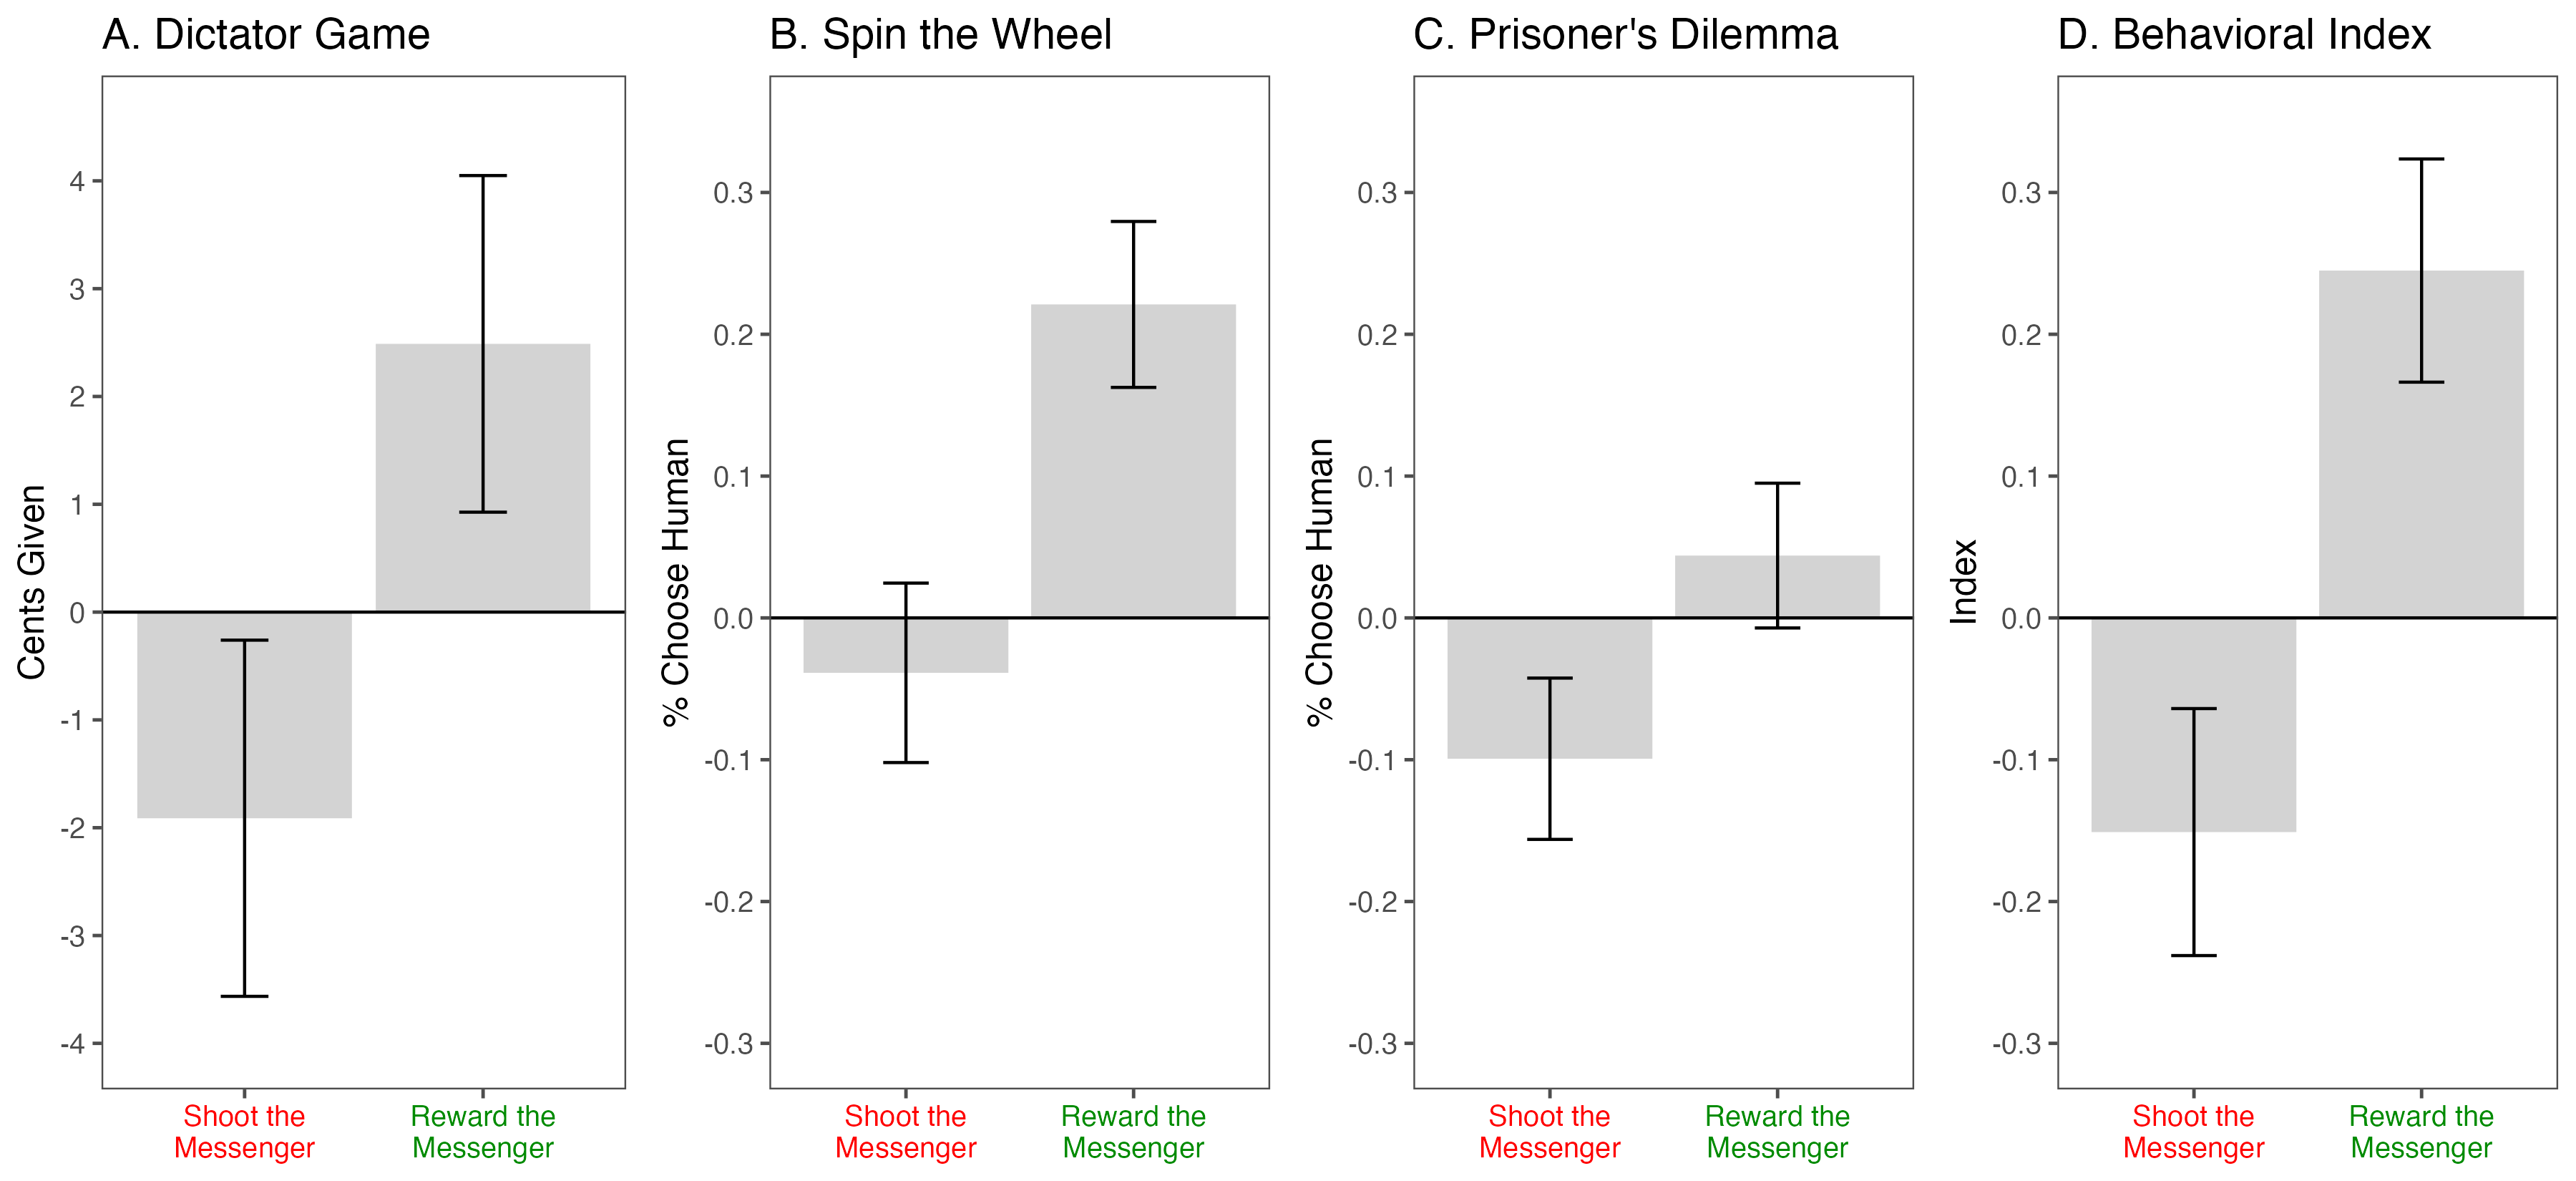
\includegraphics[width=1.0\textwidth]{figures/study1_behavior_list.png}
  \caption{Difference in the DVs of the behavior measures for messengers and non-messengers 
                                              by losing (STM) and winning (RTM), Study 1. 
  \textit{Note: OLS regression with robust standard errors, with error bars representing 95\% confidence intervals. In the dictator game (Panel A), the dependent variable (DV) is giving up to 50 cents to the partner. 
                 In the spin the wheel task (Panel B), the DV is choosing the partner to spin the wheel on one’s behalf instead of the computer. 
                 In the prisoner’s dilemma (Panel C), the DV is choosing cooperation. 
                 In the behavioral index (Panel D), the DV is calculated by averaging the standardized scores of the dictator game, spin the wheel task, and prisoner's dilemma. The p-values of the test that $RTM = -STM$ are 0.62, 0.00, 0.16, and 0.12, respectively, for each facet and the index. The p-values of messenger bias are 0.00, 0.00, 0.00, and 0.00, respectively, for each facet and the index.}}
  \label{fig:behavior_list}
\end{figure}%
\renewcommand{\baselinestretch}{1.67}%


Across all three behavioral measures, we see consistent evidence of a
messenger bias, which means participants treat messengers differently
compared to non-messengers holding constant whether the respondent wins or
loses. However, whether this bias is a result of shooting or rewarding
the messenger differs based on the specific behavioral game that the
respondents play. To start, we analyze the results of the dictator game,
where respondents could give between 0 and 50 cents to their partner
(Figure \ref{fig:behavior_list}, Panel A). We compare allocations by respondents after
winning rather than losing in decisions toward messengers and
non-messengers. When participants lost rather than won in task 1, they
sent messengers 1.91 cents less ($p < .05$) than
non-messengers, indicating that respondents ``shot the messenger''
when losing. By contrast, winning also significantly affected respondents'
behavior toward messengers compared to non-messengers (coefficient for
RTM = 2.49, $p < .01$). The difference in the relative
magnitude of these two estimates is not significant ($p =
.62$).

Next, we look at results from the spin the wheel task (Figure \ref{fig:behavior_list}, Panel B). Unlike the dictator game, we do not detect a STM effect, as 
respondents were only 4 points less likely to choose the messenger following
a first stage loss ($p = .23$). But the RTM effect persists, as when
they won in task 1, respondents were 22 points (47\%) more likely to
choose the messenger (70\%) than another participant
(48\%) ($p < .001$). We find significant
evidence of a stronger RTM effect compared to the STM effect ($p < .001$).

Finally, we look at respondents' decisions in the prisoner's dilemma
(Figure \ref{fig:behavior_list}, Panel C). When they lost in task 1, respondents were
10\% less likely to cooperate with the messenger compared to a
non-messenger ($p < .001$), providing evidence of a STM
effect. When they won in task 1, respondents were 4\% more likely to
cooperate with the messenger (79\%) than with another participant
(75\%), but this RTM effect is not significant ($p < .1$).
The difference in absolute size of these effects is not statistically
significant.

Grouping all of the behavioral measures into one combined index in
Panel D of Figure \ref{fig:behavior_list} (which we term the ``behavioral index,''
calculated as the average of the standardized behavioral measures
ranging from 0 to 1) we see an overall
STM effect of .15 and an RTM effect of .25 (both coefficients are
significant at the $p < .001$) level, which implies that
a messenger bias exists from both shooting and rewarding the messenger
($p < .001$). Although the RTM point estimate has a larger
magnitude than the STM effect, this difference is not significant ($p
= .12$). These results do not change when we include
demographic controls (Table \ref{tab:behavior_regression_demographic}).
\footnote{Along with demographic covariates such as age, gender, ideology,
education, employment, and race, we also include three psychological scales that may be
related to the messenger bias or our outcome measures. These are the just world
scale \citep{lipkus1991construction}, the emotion regulation scale \citep{buss1992aggression}, and the
belief in luck scale \citep{darke1997belief}.}
\renewcommand{\baselinestretch}{1.25}%
\begin{figure}[!t]%
  \centering
  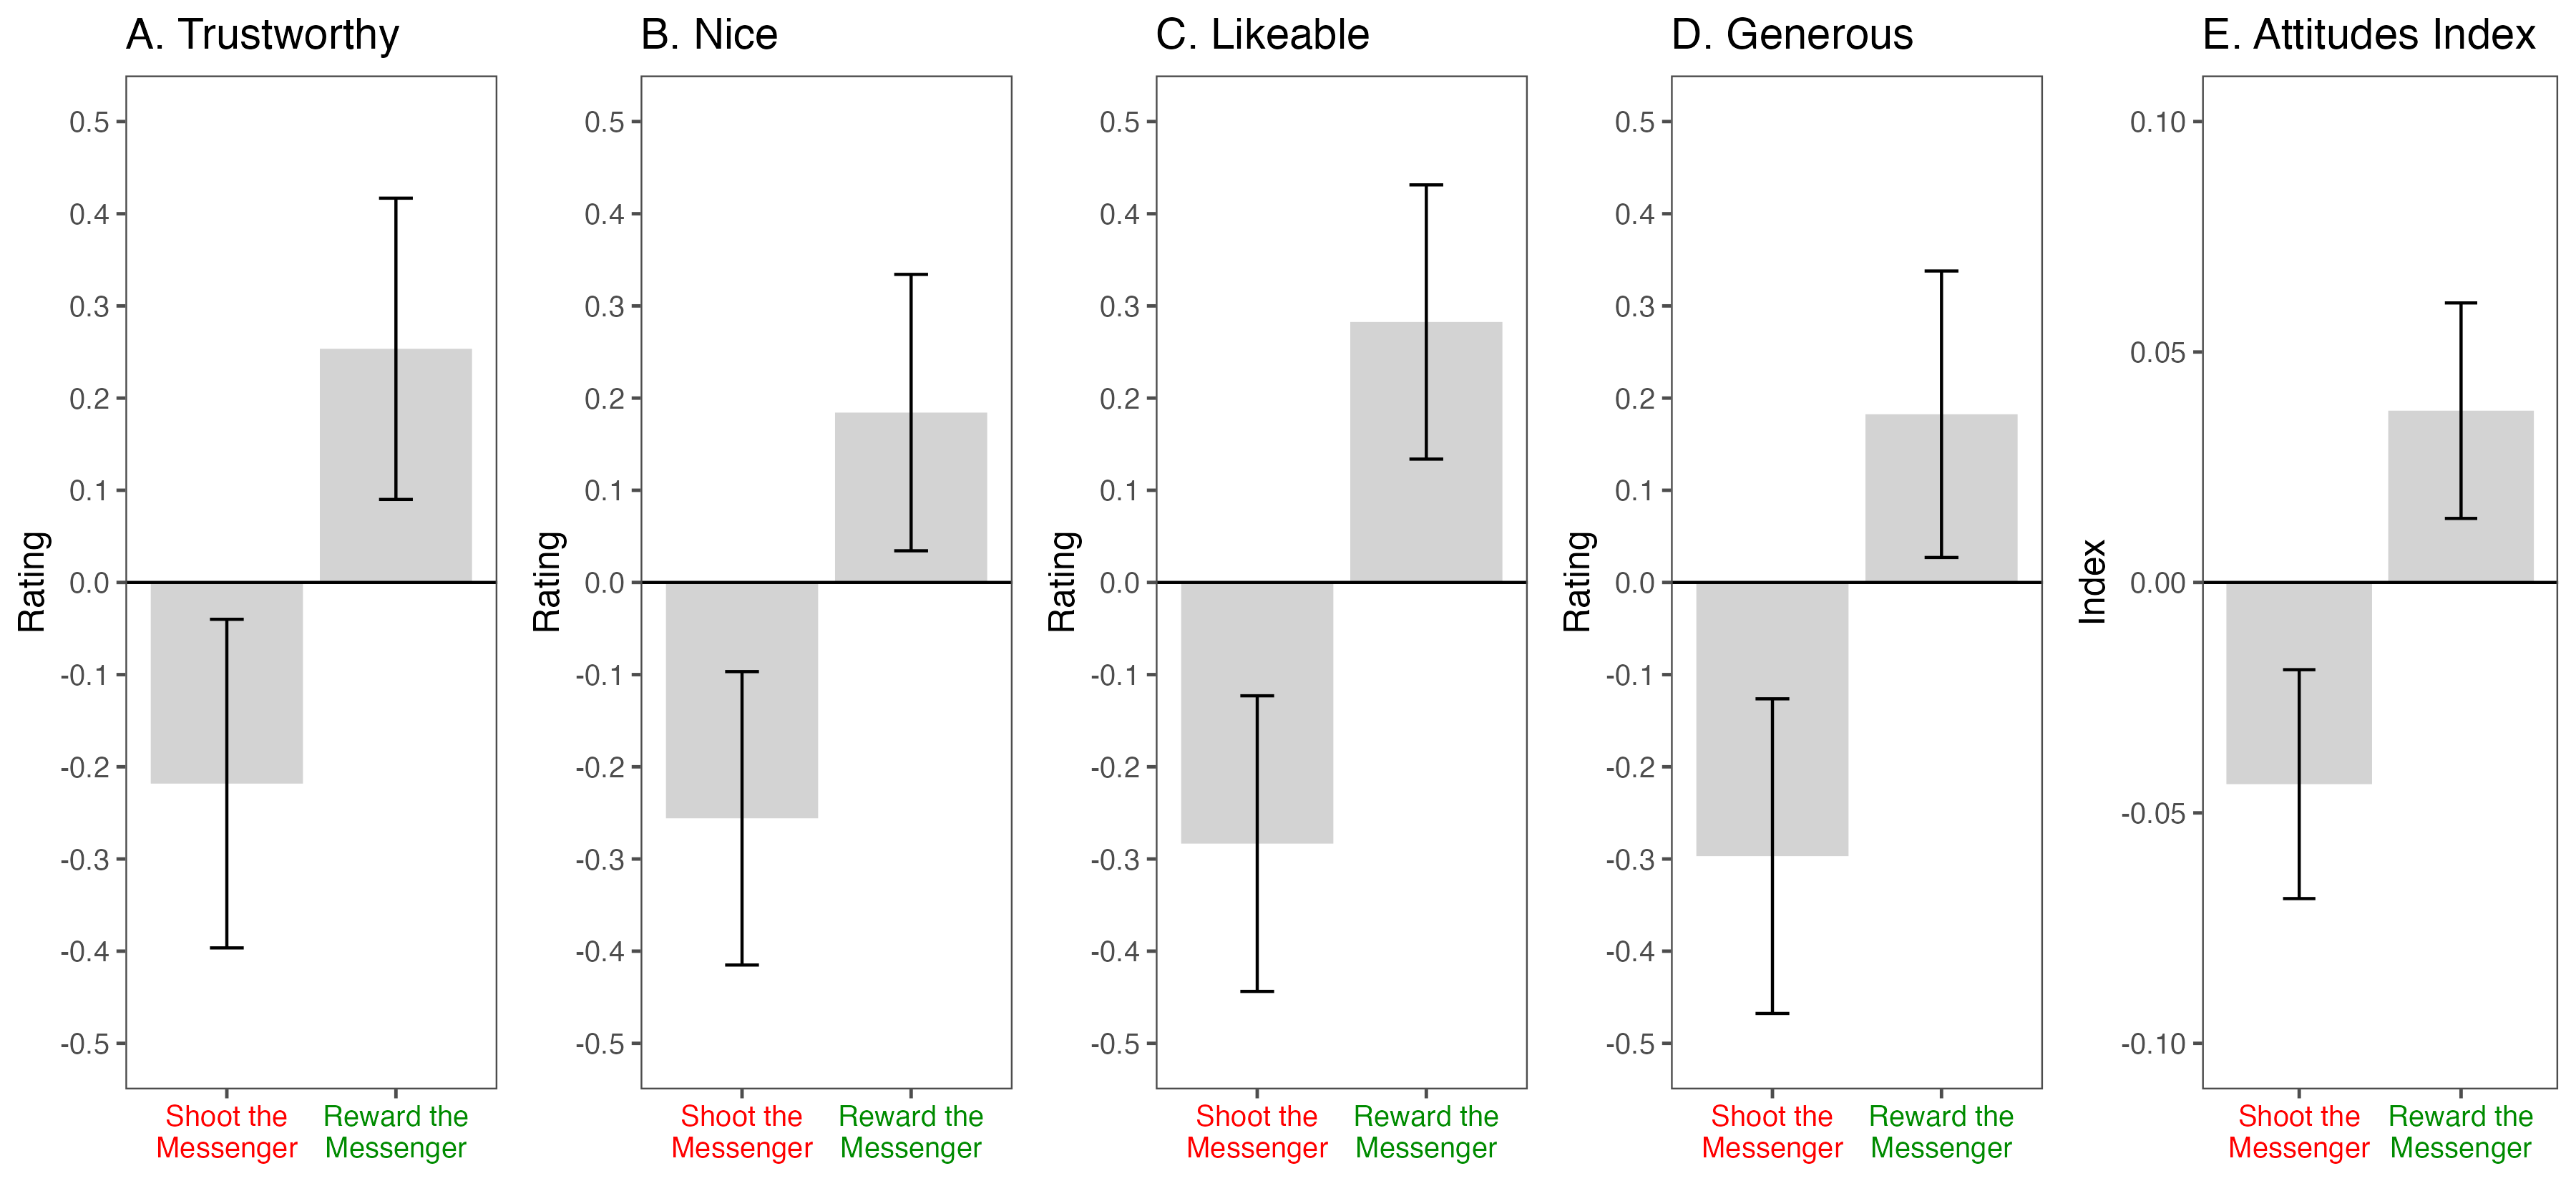
\includegraphics[width=1.0\textwidth]{figures/study1_attitude_list.png}
  \caption{Difference in the DVs of the attitude measures for messengers and non-messengers 
                                              by losing (STM) and winning (RTM), Study 1. 
  \textit{Note: OLS regression with robust standard errors, with error bars representing 95\% confidence intervals. The trustworthy (Panel A), nice (Panel B), likeable (Panel C), and generous (Panel D) dependent variables asks respondents to rate these messenger's characteristics on a 7-point Likert scale, where a score of 1 indicates that the messenger does not have that trait at all, while a score of 7 means that a trait describes the messenger extremely well.
    In the attitudes index (Panel E), the DV is calculated by averaging the ratings of the trustworthy, nice, likeable, and generous DVs to an index ranging from 0 to 1. The p-values of the test that $RTM = -STM$ are 0.77, 0.52, 0.99, 0.33, and 0.71, respectively, for each facet and index. The p-values of the messenger bias are 0.00, 0.00, 0.00, 0.00, and 0.00, respectively, for each facet and the index.}}
  \label{fig:attitude_list}
\end{figure}%
\renewcommand{\baselinestretch}{1.67}%


Next, we analyze the four attitudinal measures (trustworthiness,
niceness, likability, and generosity). Figure \ref{fig:attitude_list} presents the results
graphically, following the same logic as Figure \ref{fig:behavior_list}. Each of these
attitudes was measured on a 7-point scale. Unlike the behavioral
measures, we see consistent messenger bias, both RTM and STM effects,
across all attitudinal measures. For simplicity, therefore, we focus on
the index measure (called the ``attitudes index,'') which averages the
 ratings of the four attitudes from 0 to 1. We
see that respondents consistently rewarded the messenger, as they are
around 4\% ($p < .01$) more favorable (for the
index measure) after winning, compared to attitudes towards the
non-messenger. Similarly, respondents consistently shot the messenger,
as they are 4\% ($p < .01$) less favorable to
messengers after losing. These effects are of equal size and
statistically indistinguishable.\footnote{We also consider more complex regression models where we include as predictors the type of task (the skill counting task or the luck prediction task) and its interactions with losing and the messenger (see Appendix \ref{sec:appendix_study1}, Table \ref{tab:behavior_regression_counting} and \ref{tab:attitude_regression_counting}). These analyses reveal that there are almost no differences in the STM and RTM effects by the type of task, with the exception of the RTM effect for behaviors being smaller for the counting (skill) task compared to the prediction (luck) task in Table \ref{tab:behavior_regression_counting}. Finally, we note that whether the message was emotional or neutral also made no difference in the behavioral outcome measures (see Appendix \ref{sec:appendix_study1}, Table \ref{tab:behavior_regression_emotional} and \ref{tab:attitude_regression_emotional}), so we also ignore that difference in our analyses here.}

To summarize, we find that respondents displayed a biased response to
the messenger in both their behaviors and attitudes, showing evidence of
a messenger bias, even though the respondents were told that the
messenger was merely mechanically reporting the participant's result for
the task. After winning, we find consistent indications of greater
altruism, trust, and (to a lesser extent) cooperation toward the
messenger compared to non-messengers. We find the opposite effect to be
true after losing: respondents ``shot the messenger'' compared to the
non-messenger in all of our behavioral measures except for the
spin-the-wheel task. For all four measures of attitudes
(trustworthiness, likeability, niceness, and generosity), we find more
consistent results. Respondents rate messengers higher after winning, and
lower after losing, compared to non-messengers. Also, in aggregate, we
note that the messenger's tone (emotional or neutral) did not affect
respondents' attitudes or behaviors, and neither did the nature of the
task that participants performed (prediction or count).

Therefore, there are two main conclusions from Study 1. First, we confirm
the presence of STM and RTM effects, with the RTM effect being equal to
or larger than the STM effect. This shows that in studying the messenger
bias, we cannot assume that the RTM effect is symmetric to the STM
effect. Second, the behavioral measures show more inconsistent
measurements of the messenger bias compared to attitudinal measures, as
we fail to find a STM effect for the spin the wheel task (a measure of the hot hand fallacy, or an intuition that the messenger can be trusted to bring good news again) and a
RTM effect for the prisoner's dilemma (a measure of cooperation). This suggests the
importance of behavioral analysis in the study of conflict and
cooperation in place of purely attitudinal outcomes, as biased attitudes
might not necessarily translate to differences in behaviors towards
messengers \citep{del2020behavioral, ostrom1998behavioral}.

\subsection{Study 2}

Study 1 documented a messenger bias in both attitudes and behaviors,
which occurred both when the messenger brought good news and when they
announced bad news. However, Study 1 left unstated whether the messenger
had any stake in the outcome of the task, despite that fact that they
had no control over it. The messenger's compensation might be important
if respondents' behaviors and attitudes depend on whether they believe that
messengers may have an \emph{interest} in conveying good news or bad
news. To address this issue, in Study 2, we specified the messenger's
stake in delivering the good or the bad news. Specifying the messenger's
stake in the news also allows us to manipulate whether the messenger's
motives are neutral (unrelated fate), aligned with (shared fate), or
opposite (opposite fate) to the ones of the participant. Manipulating
the messenger's incentives may provide insights into whether the
messenger bias can be reduced or strengthened depending on the alignment
of the messenger's stakes, which allows us to understand if
institutional designs can counteract the behavioral tendency to treat
messengers differently depending on the news they deliver.

Similar to Study 1, we analyzed the results of losing and winning in the first task on behaviors and attitudes towards messengers and non-messengers by the three treatment conditions: shared, unrelated, and opposite Fate. For simplicity, we present only the behavioral and attitudes
indices in Figures \ref{fig:study2_main_behavior_all} and \ref{fig:study2_main_attitude_all} (the associated regression
tables are in Appendix \ref{sec:appendix_study2}). Unlike in the presentation of the Experiment
1 results, the first three columns or facets of each figure are for the
three conditions in Study 2 (shared fate, unrelated fate, and opposite
fate). The last column repeats the index dependent variable from
Study 1 for reference, in which respondents were not explicitly told about any
incentives for the messenger.

\renewcommand{\baselinestretch}{1.25}%
\begin{figure}[!t]%
  \centering
  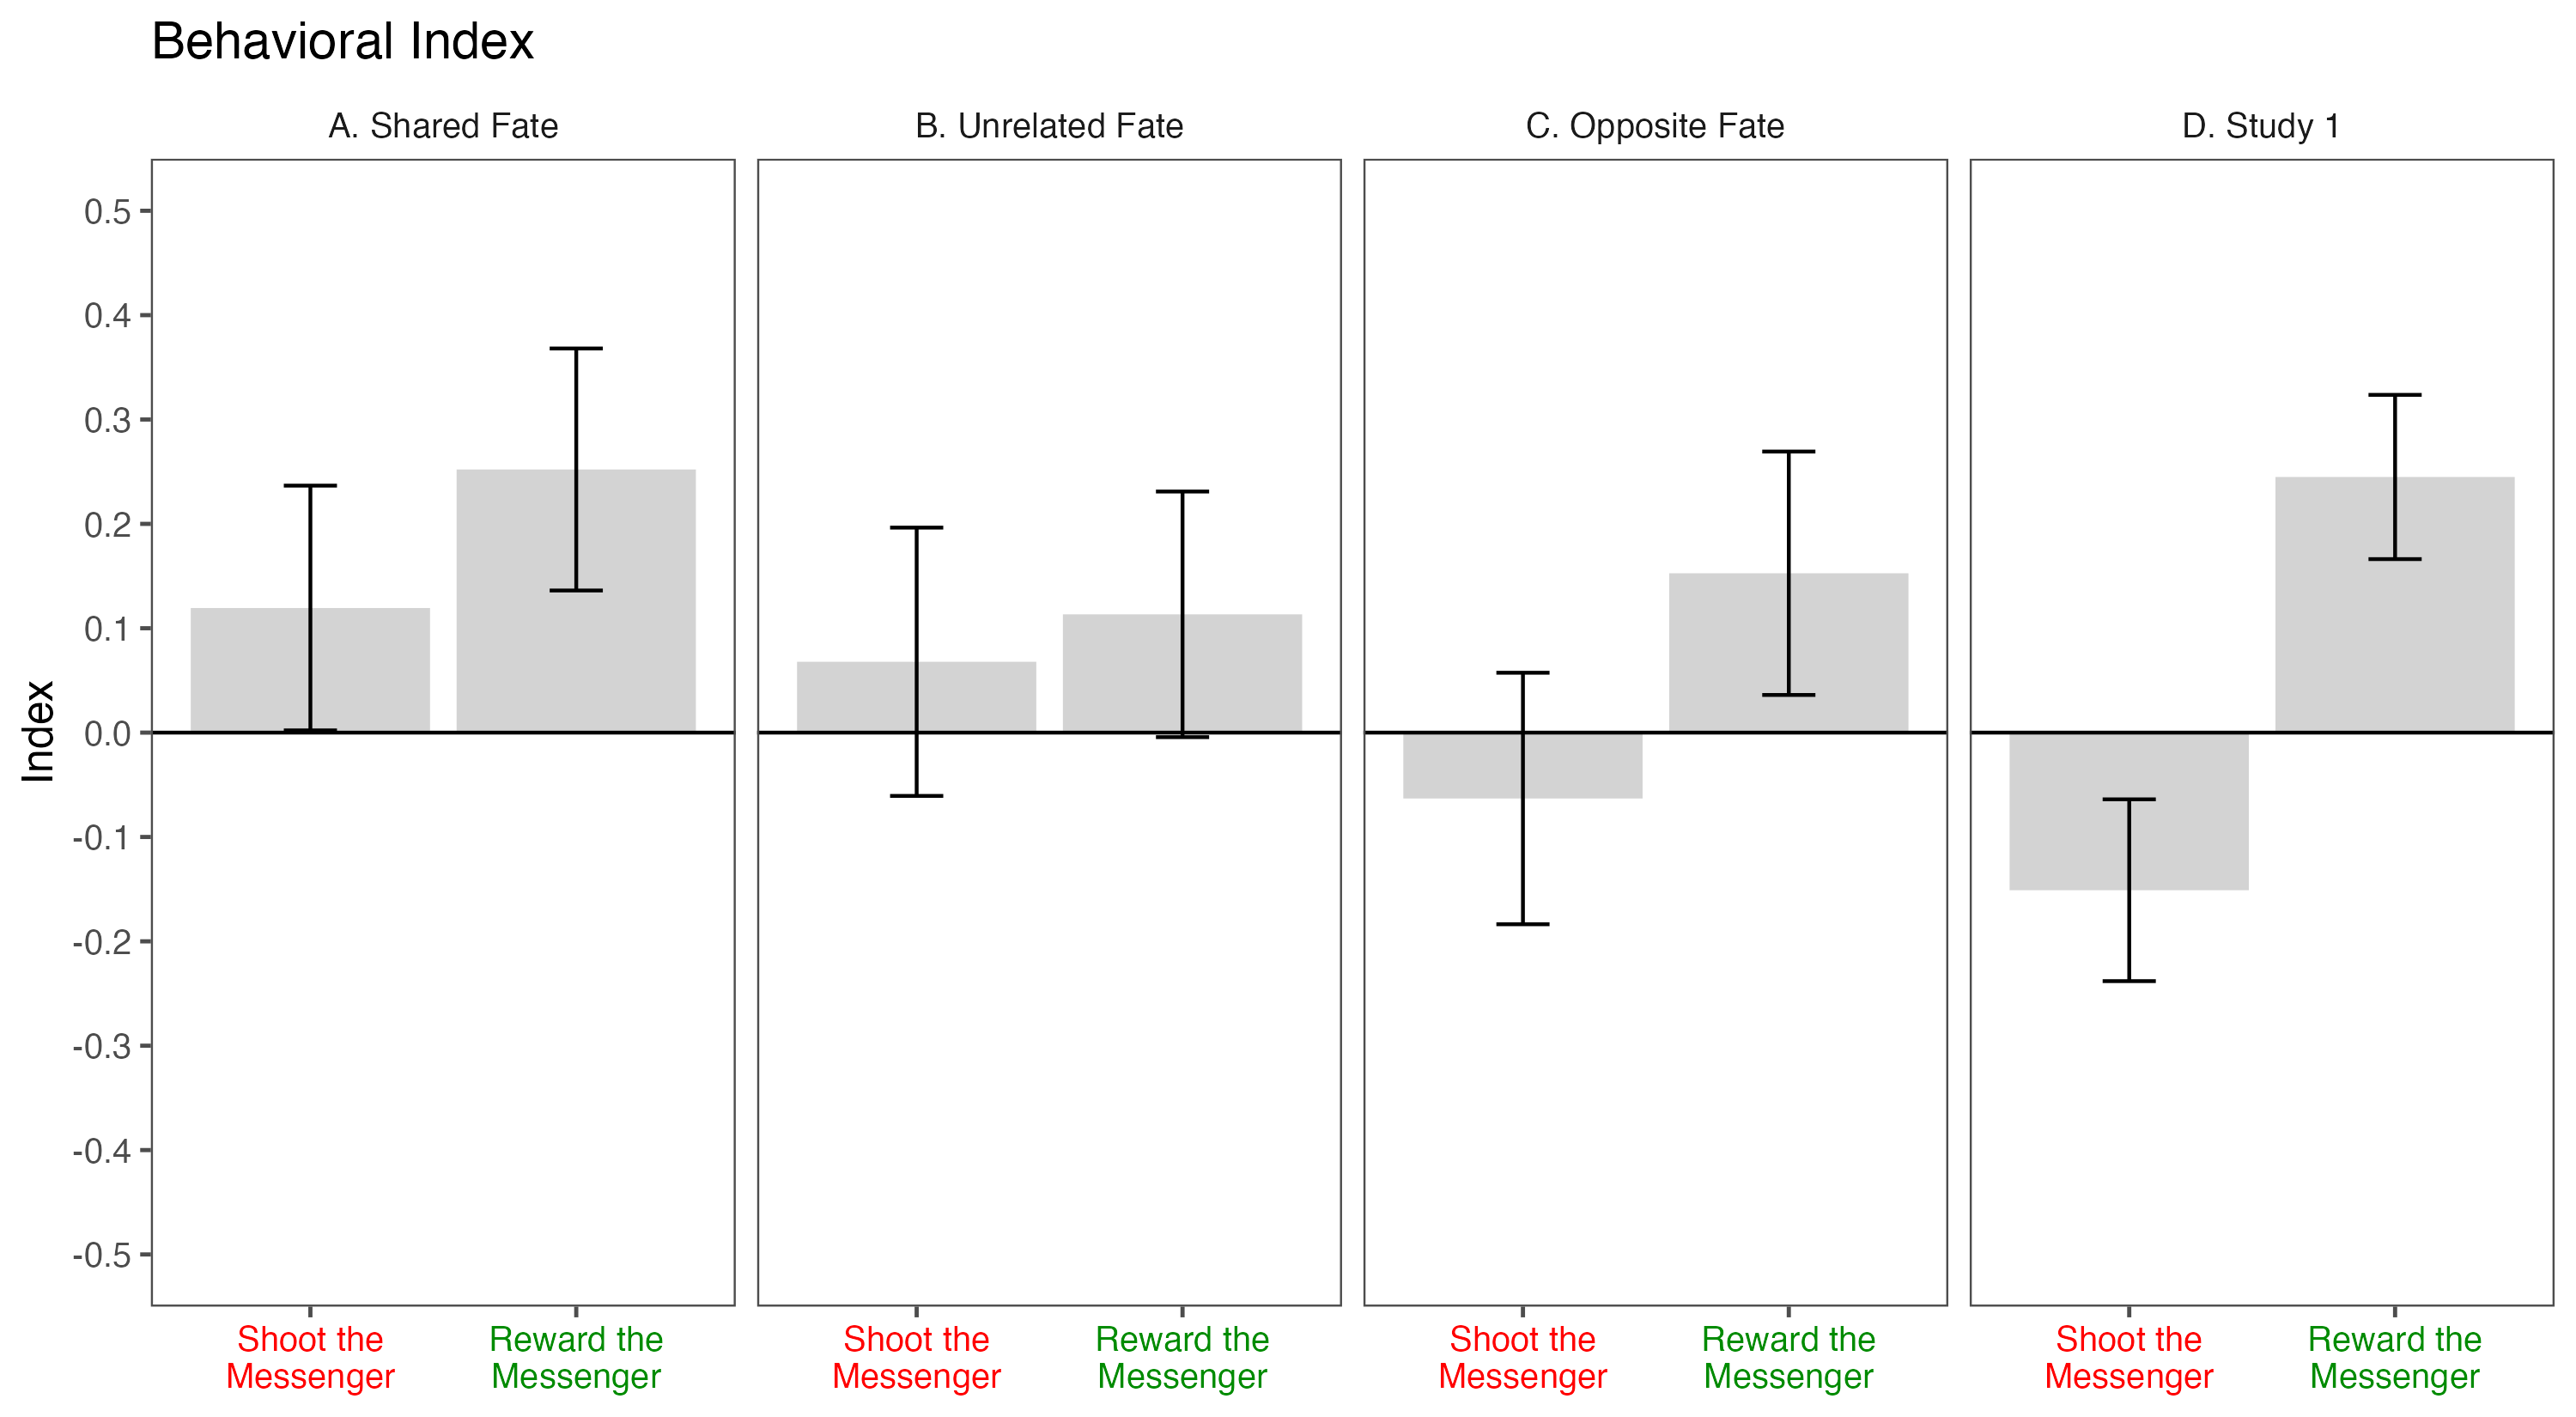
\includegraphics[width=1.0\textwidth]{figures/study2_main_behavior_all.png}
  \caption{Difference in messenger and non-messenger ratings of the Behavioral Index by losing (STM) and winning (RTM) across Unrelated Fate, Shared Fate, Opposite Fate conditions, Study 2. 
  \textit{Note: OLS regression with robust standard errors, with error bars representing 95\% confidence intervals.In the behavioral index, the DV is calculated by averaging the standardized scores of the dictator game, spin the wheel task, and prisoner's dilemma. The Shared Fate (Panel A), Unrelated Fate (Panel B), and Opposite Fate (Panel C) conditions are when the partner wins when the respondent wins, the partner winning are unrelated to the respondent winning, and the partner wins when the respondent loses, respectively. Study 1 (Panel D) repeats the index measure from Study 1 as a reference, where respondents were not explicitly given the alignment of their partner. The p-values of the test that $RTM = -STM$ are 0.00, 0.04, 0.29, and 0.12, respectively, for the Shared, Unrelated, Opposite Fate conditions, and Study 1. The p-values of the messenger bias are 0.00, 0.1, 0.02, and 0.00, respectively, for the Shared, Unrelated, Opposite Fate conditions, and Study 1.}}
  \label{fig:study2_main_behavior_all}
\end{figure}%
\renewcommand{\baselinestretch}{1.67}%


First, we analyze the effect of winning (reward the messenger) and
losing (shoot the messenger) on the behavioral index in Figure \ref{fig:study2_main_behavior_all}, which allows us to
test whether these conditions eliminate the messenger bias. Across all
three conditions (and similarly to Study 1), we find that the
reward the messenger (RTM) effect remains, although it is not
significant in the unrelated fate condition ($p = .06$). However, we
see that the shoot the messenger (STM) effect is eliminated entirely in
the shared and unrelated fate conditions and attenuated substantially in
the opposite fate condition. In the unrelated fate condition, the STM
effect is positive but not significantly different than 0, although it
is negative but not significant in the opposite fate condition (about
33\% of the estimated effect from Study 1). Finally, the shared
fate condition reverses the STM effect completely---telling the
respondents that the messenger shares their positive or negative outcome
causes respondents to behave in a prosocial manner towards the
messenger, regardless of whether they win or lose. Thus, when comparing
the relative magnitude of the RTM and STM effects, we find that the RTM
effect is significantly larger than the STM effect in the shared and unrelated fate conditions.
Overall, we find evidence that the messenger bias disappears completely
only in the unrelated fate condition, which shows that specifying that
the messenger's outcomes are not related to the respondent's is
effective in getting rid of either positive or negative bias towards the
messenger.

\renewcommand{\baselinestretch}{1.25}%
\begin{figure}[!t]%
  \centering
  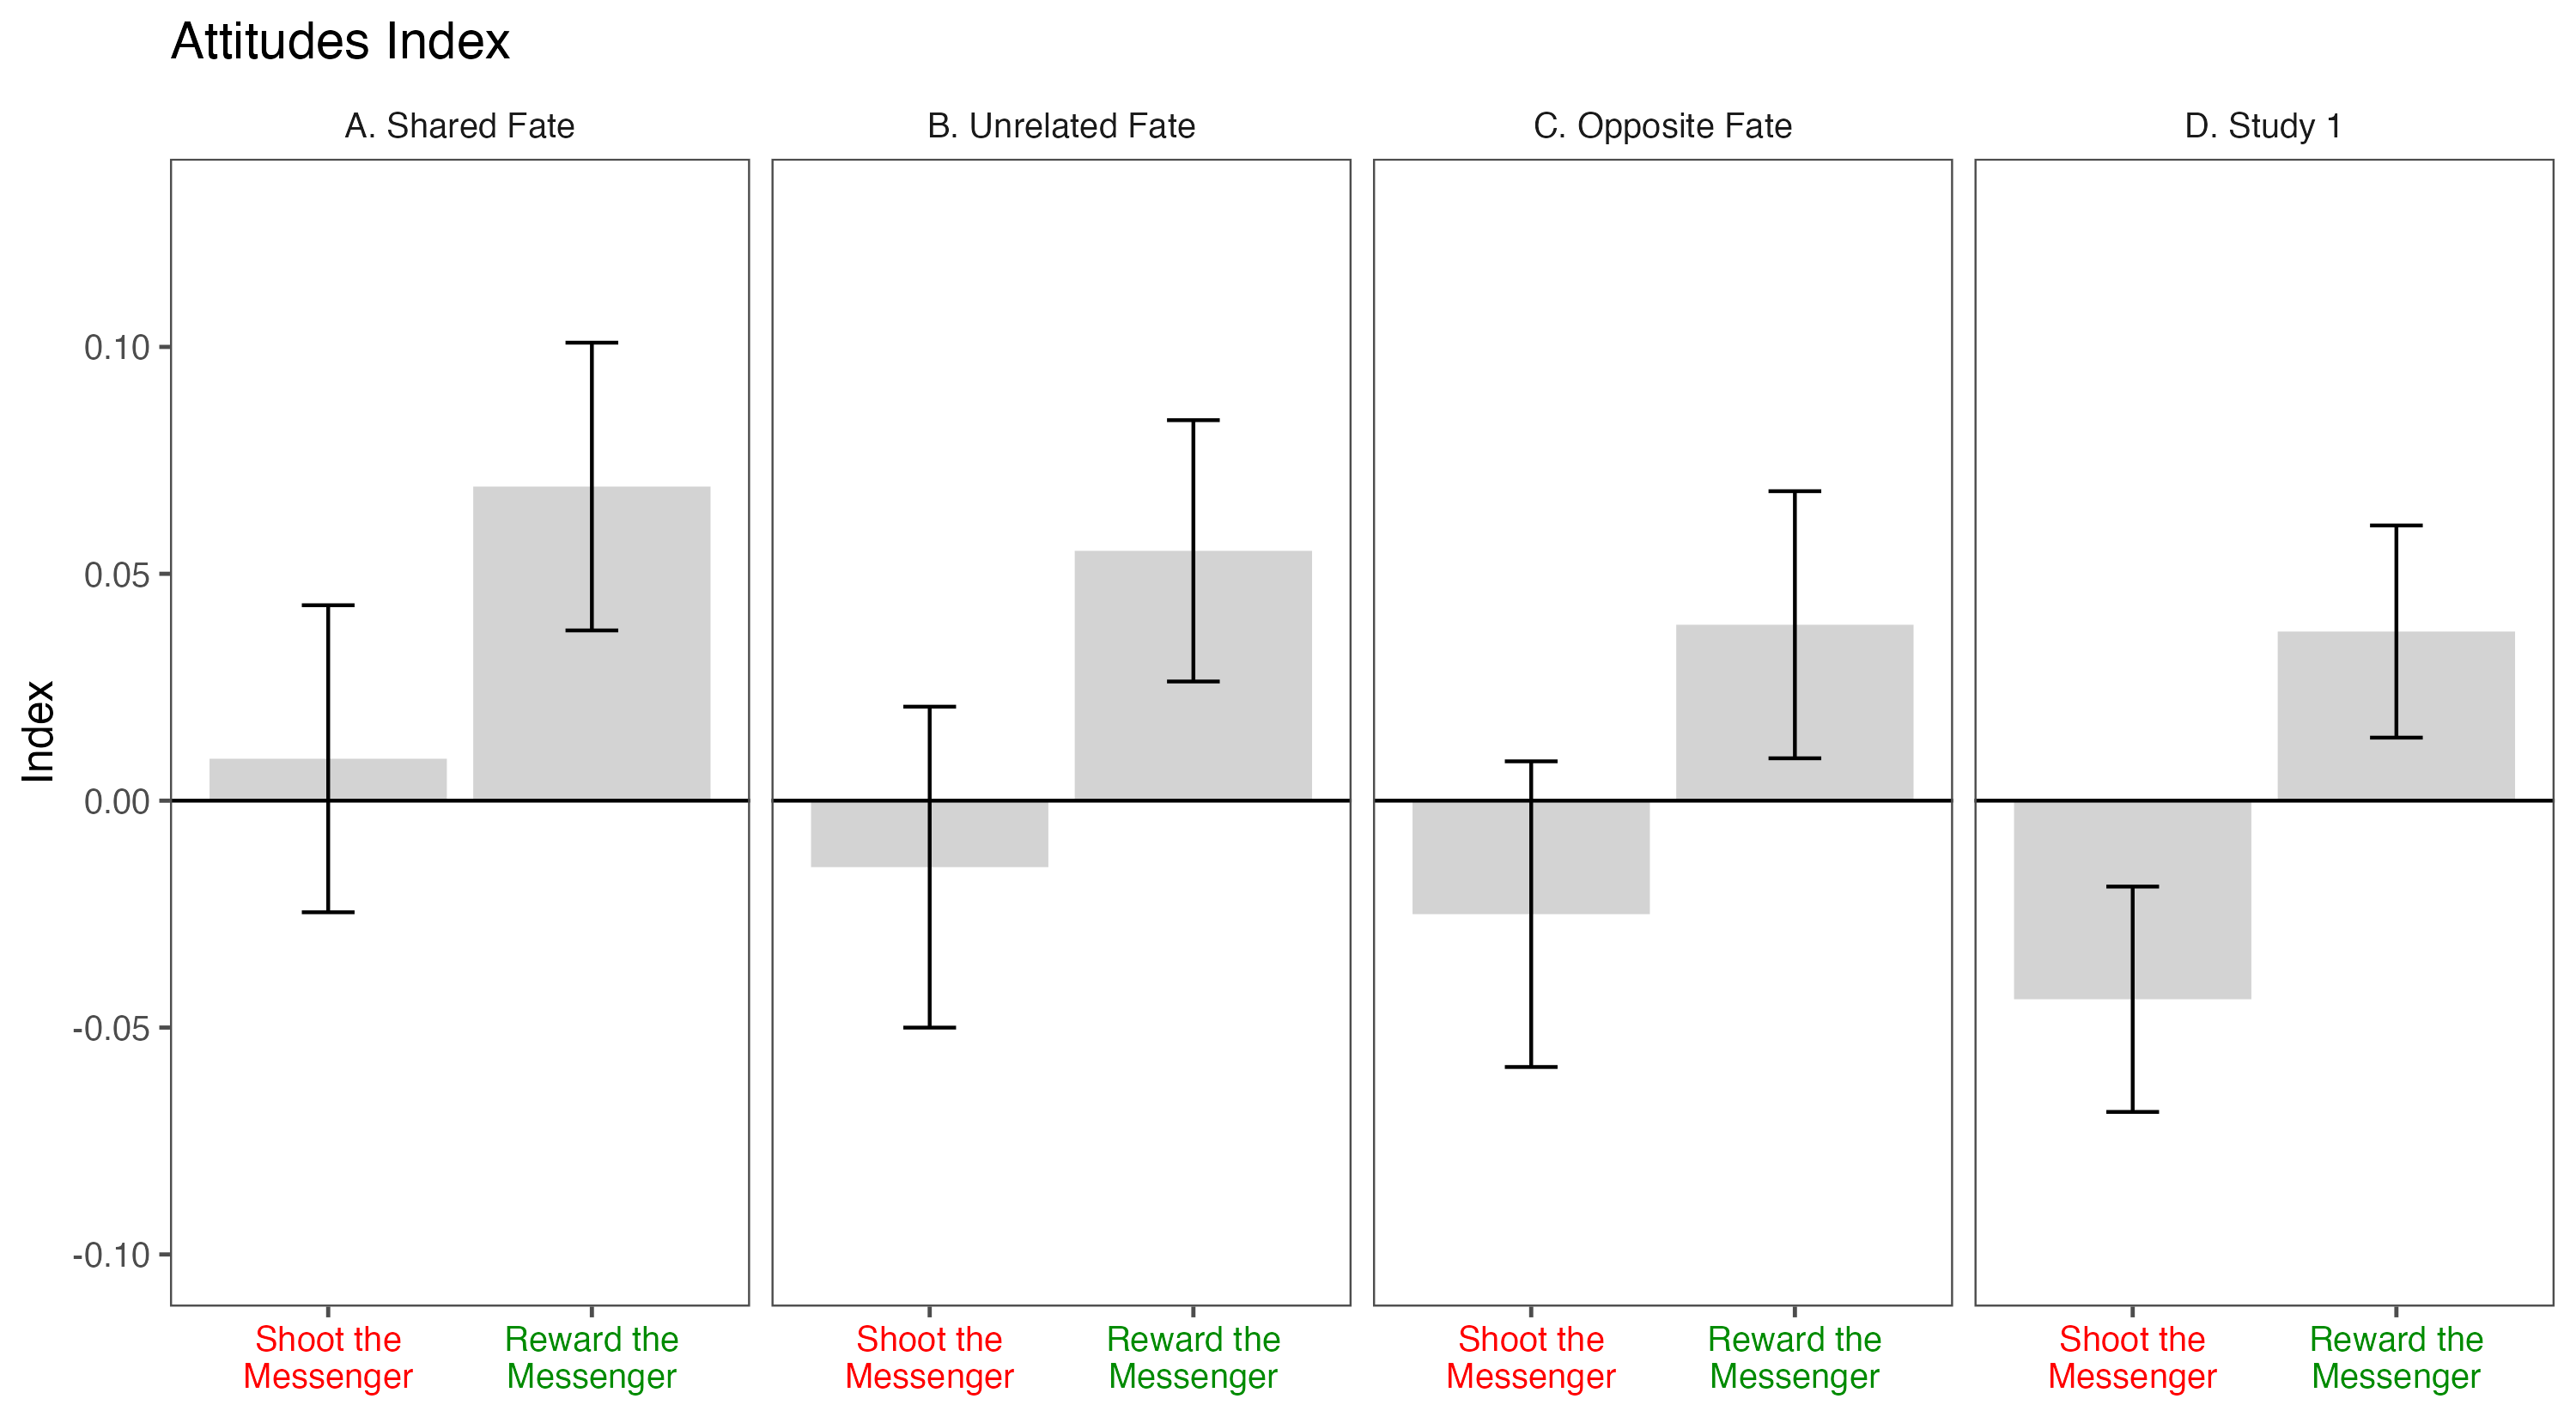
\includegraphics[width=1.0\textwidth]{figures/study2_main_attitude_all.png}
  \caption{Difference in messenger and non-messenger ratings of the Attitudes Index by losing (STM) and winning (RTM) across Unrelated Fate, Shared Fate, Opposite Fate conditions, Study 2. 
  \textit{Note: OLS regression with robust standard errors, with error bars representing 95\% confidence intervals.In the attitudes index, the DV is calculated by averaging the ratings of the trustworthy, nice, likeable, and generous DVs to an index ranging from 0 to 1. The Shared Fate (Panel A), Unrelated Fate (Panel B), and Opposite Fate (Panel C) conditions are when the partner wins when the respondent wins, the partner winning are unrelated to the respondent winning, and the partner wins when the respondent loses, respectively. Study 1 (Panel D) repeats the index measure from Study 1 as a reference, where respondents were not explicitly given the alignment of their partner. The p-values of the test that $RTM = -STM$ are 0.00, 0.08, 0.55, and 0.71, respectively, for the Shared, Unrelated, Opposite Fate conditions, and Study 1. The p-values of the messenger bias are 0.00, 0.00, 0.01, and 0.00, respectively, for the Shared, Unrelated, Opposite Fate conditions, and Study 1.}}
  \label{fig:study2_main_attitude_all}
\end{figure}%
\renewcommand{\baselinestretch}{1.67}%


Next, we analyze the attitudes index in Figure \ref{fig:study2_main_attitude_all}. As with the behavioral index, we
see that the RTM effect persists across all three conditions, although
it is lowest in the opposite fate condition and highest in the shared
fate condition. We also see that the STM effect is not statistically
significant in any condition, although it also monotonically decreases
from the opposite to the shared fate conditions. The point estimate is
positive only in the shared fate condition. As with the behavioral
index, the RTM effects are again significantly larger than the STM
effects in the shared and unrelated fate conditions. However, no condition eliminated the
messenger bias for the attitudinal measures, which implies that
respondents were much more likely to view messengers positively when
they delivered good rather than bad news.

Overall, in Study 2, we find three important results. First, we continue
to find that the STM and RTM effects for behaviors are different than
those for attitudes, even when we specify the fate of the messenger.
Although it may be possible to eliminate the messenger bias for
behaviors, we find no such result for attitudinal measures. Second,
whether the incentives of messenger and respondent are aligned or
misaligned is crucial for determining whether messenger bias arises.
Across all conditions and measures, specifying the stakes of the
messenger in the outcome reversed the sign of or attenuated the STM
effect. In contrast, the RTM effect was present across most conditions
for both behaviors and attitudes. The only exception was the unrelated
fate condition, which was the only treatment to eliminate the messenger
bias completely
for behavioral measures, as we find no STM or RTM effects. Surprisingly,
the shared fate condition induced respondents to reward the messenger regardless of whether
the respondent won or lost: clarifying that the messenger had the same
stakes as the participant elicited more positive behaviors towards
messengers even after losing. Finally, RTM effects were asymmetric to
STM effects. RTM effects are especially persistent across most treatment
conditions and larger than STM effects, which is further evidence from
Study 1 that the RTM and STM effects are not symmetric and deserve to
be examined in turn. We expected the shared (opposite) fate condition to
eliminate (exacerbate) the STM effect and exacerbate (eliminate) the RTM
effect. While we do find this for the shared fate condition, we do not for the opposite fate condition: the STM effect reverses sign in some
conditions, but is still attenuated in the opposite fate condition. In contrast, RTM
effects are persistent across most conditions, even when the messenger has the
opposite incentives of the respondent. This finding points to a fruitful avenue for additional research: What incentives do respondents assume a messenger has when they are not specified?

\section{Discussion}

Across two incentivized experiments with thousands of participants, we
find consistent evidence of the messenger bias and how to mitigate it.
In Study 1, participants both shot and rewarded the messenger for
delivering bad news and good news, respectively. In Study 2, the
STM effect was either eliminated entirely or substantially diminished
across all conditions for both attitudes and behavioral measures when
clarifying the stakes the messenger had in the outcome. Specifically,
when the messenger clarified their (non-)stakes in the outcome
(unrelated fate), participants did not dislike the messenger more and
did not treat the messenger better or worse than a non-messenger. In the
shared and opposite fate conditions, the RTM effect persisted for both
attitudinal and behavioral measures. When incentives were aligned
(shared fate conditions), both the RTM and STM effects were positive, as
respondents behaved more prosocially regardless of whether they won or
lost. When incentives were misaligned (opposite fate conditions),
participants still consistently rewarded messengers delivering good
news but failed to punish messengers for delivering bad news.

Our paper contributes three new findings to the literature. First, we go
beyond the prior exclusive focus on the STM effect and look at both the
STM and RTM effects together. The STM effect may be a major source of
inefficiency in society because messengers know that backlash may await
them after communicating bad news. Moreover, in an environment where
messengers know that they face punishment for breaking bad news and
rewards for conveying good news, messengers have incentives to alter or
withdraw news. Thus, information cannot be easily trusted, possibly
breeding inefficiencies and a decline in cooperation in the absence of
strategies or institutions that restore incentives for messengers to
tell the truth. However, we also find that the RTM effect is greater
than or equal to the STM effect and surprisingly resilient in Study 2
compared to the STM effect. The RTM effect is just as normatively concerning
and deserving attention because it suggests people may rush to convey
good news regardless of whether they contributed to the good outcome. At
one extreme, people's intuitions to reward pure messengers may skew the
incentives in the communication environment from producing good news to
communicating it. This may be undesirable because it puts the creators
of good outcomes for society at a relative disadvantage compared to the
people who communicate those outcomes to the public, such as influencers
on social media or spokespersons.

Second, the present experiments provide the first evidence of a
messenger bias that affects prosocial behavior and goes beyond
attitudes. When no information about the messenger's payoffs was
provided in Study 1, respondents' attitudes toward the messenger
indicated that they rate the messenger to be less trustworthy, nice,
likeable, and generous after losing and the opposite after winning. Yet,
behavioral measures show that this does not extend to acting less
trusting after losing (shooting the messenger for spin the wheel) or
more cooperative after winning (rewarding the messenger for prisoner's
dilemma). Study 2 confirms this discrepancy between behavioral and
attitudinal measures, as the unrelated fate condition was able to
eliminate the messenger bias completely for behavioral measures, but the
messenger bias persisted for attitudinal measures across all conditions.
Therefore, only focusing on attitudinal measures like prior work would
overestimate the impact of the messenger bias, as biased attitudes may
not translate into biased behaviors towards the messenger. This study
demonstrates the importance of using behavioral measures to better
understand the implications of the messenger bias and how to reduce it.

Finally, we show one effective strategy that broadly eliminates STM
effects for biased behaviors: specifying the incentives of the messenger
in the message outcome. Our second experiment was effective in broadly
reducing the STM effect for cooperation, altruism, and trust toward
messengers, along with attitudinal measures. Yet, a limitation of our
current research is that we only somewhat ameliorated the RTM effect (for the unrelated fate condition for behaviors), and even
exacerbated it with the shared fate conditions. This may still be
problematic as individuals were rewarded for mechanically announcing
good news which they did not create. While we identify one potential
strategy to ameliorate the RTM and STM effects, future research should
explore other effective strategies beyond clarifying the relationship
between the messenger and the message. These could involve avoiding using
controlling or abstract messages \citep[see, e.g.,][]{sparks2008style,miller2007psychological} or increasing messenger credibility \citep[see, e.g.,][]{hunt1984role,kamins1987twosided}. 
Future work can then
continue to unravel the messenger bias and its impact on interpersonal
relations, markets, and politics, along with how to mitigate these
impacts.
